\documentclass[12pt,letterpaper]{article}

% Librerías a utilizar
\usepackage[utf8]{inputenc}	% Codificación 
\usepackage[spanish]{babel}	% Idioma
\usepackage{graphicx}		% Imagenes
\usepackage{indentfirst}		% Sangría
\usepackage{amsmath, amsfonts, amssymb}	% Figuras matemáticas
\usepackage{url}    % URL
\usepackage{dutchcal}
\newcommand{\subsubsubsection}[1]{\paragraph{#1}\mbox{}\\}
\setcounter{secnumdepth}{4}
\setcounter{tocdepth}{4}


\usepackage[left=3cm,right=2cm,top=2cm,bottom=3cm]{geometry}

\setlength{\parindent}{2cm}	% Sangría en los párrafos
\renewcommand{\baselinestretch}{1.5}	% Interlineado

% Renombrar ciertos títulos del texto
\renewcommand\spanishcontentsname{Tabla de contenidos}


% Inicio del documento
\begin{document}

%%%%%%%%% PORTADA %%%%%%%%%

\newpage
\vspace*{-.5cm}
% Logo institucional
\begin{picture}(18,4)(0,30)
	\put(350,-20){
\includegraphics[scale=0.25]{./imagenes/LogoUsach.pdf}}
\end{picture}

\sloppy
\thispagestyle{empty}
\vspace*{-1.6cm}

% Datos institucionales
\begin{center}
	{\bf \mbox{\large UNIVERSIDAD DE SANTIAGO DE CHILE}}\\
	{\bf \mbox{FACULTAD DE INGENIER\'IA}}\\
	{\bf \mbox{DEPARTAMENTO DE INGENIER\'IA INFORM\'ATICA}}\\
\end{center}

	\vspace{5cm}
	%Título del trabajo
	\begin{center}
	\Large
		\textbf{Informe de Algoritmos numéricos: \\ Laboratorio II}{  }
	\end{center}
	
	% Datos personales
	\vspace*{6.25cm}
	\begin{flushright}
		\begin{tabular}[t]{l l}
			Integrante: &Alberto Rodríguez\\			
			Curso: &Algoritmos numéricos\\
			Sección &0-L-2\\
			Profesor(a): &Óscar Rojas Díaz

		\end{tabular}
	\end{flushright}
	\begin{center}
		\vspace{1.5cm}
		% Fecha
		\Today
	\end{center}

\newpage
\tableofcontents
\thispagestyle{empty}

\newpage
\listoffigures
\thispagestyle{empty}

\newpage
\listoftables
\thispagestyle{empty}

\newpage
\renewcommand{\thepage}{\arabic{page}}
\setcounter{page}{1}

% Capítulos agregados 
% Capítulos agregados 
\section{Introducción}

\par En la actualidad todo gira en torno a los números y diversos cálculos matemáticos, para esto se realizan distintos tipos de operaciones. Por lo mencionado anteriormente, es que se usa una rama de la matemática llamada análisis numérico, que mediante distintos tipos de métodos numéricos se realizan cálculos y a su vez un completo análisis de estos resultados obtenidos.

\par Un buen uso de los métodos numéricos otorga una infinidad de habilidades, las cuales pueden ser ocupadas en el día a día. Sin embargo, el problema que ocurre es que la computadora no puede aprender ciertas habilidades, por el simple motivo de no tener la capacidad pensante del humano. Debido a esto es que se ocupan técnicas para disminuir la dificultad de los distintos métodos numéricos, algunas  de las más utilizadas es la aproximación.

\par El desarrollo del presente laboratorio se divide en dos partes las cuales son categorizadas como: Calculo de una integral definida mediante 3 formas de calculo para esta, y la aplicacion de un método o tecnica para resolver una ecuacion difernecial parcial.

\subsection{Objetivos}

\par El objetivo que busca dicho laboratorio, es aplicar cada uno de los métodos de calculo de la intregal para la Parte I, y resolver con algun metodo la ecuacion diferencial parcial de Cromatografia de Membrana para la Parte II. Para ello se deben diseñar algoritmos capaces de entregarmel resultado aproximado de los calculos.

\subsection{Herramientas}

\par Las herramientas ocupadas para el desarrollo del laboratorio e informe fueron las siguientes.

\begin{enumerate}
	\item Para la realización del código fuente de ambas partes se ocupó Matlab R2918b.
	\item  Para la realización de la documentación del laboratorio se ocupó Latex-Texstudio 
\end{enumerate}



 
\section{Parte I}

\subsection{Problema}

\par Se solicita implementar un algoritmo para una integracion adaptativa, esta consiste en aproximar la integral L(f) dividiendo la integral en subintervalos, esta definida en entre los intervalos [a,b] y se realiza la  división de intervalo de m=(a+b)/2. Para este laboratorio la funcion a evaluar es (1):

\begin{equation}
	L(f) = \int_{a}^{b} 2^{x} - 4x\cdot dx
\end{equation}

\par Se debe determinar la cantidad de iteraciones segun una toleracia de error \textit{tol}, además obtener el error obtenido en la ultima iteración. Los intervalos [a,b] y la tolerancia son ingresados como parametros.

\par Para el desarrollo del calculo de la integral se deben utilizar 3 formas de calculo de integral: 

\begin{enumerate}
	\item Trapecios simples
	\item Integracion de Simpson 1/3
	\item Integracion de Simpson 3/8
\end{enumerate}

\par Para poder realizar los calculos se debe tener un buen conocimiento de como funcionan estos métodos. Al final ya obtenidos los resultados de la integral, iteraciones y error de cada método, se debe incluir gráficas y tablas de evalucacion de errores, comparando los resultados de cada método anteriormente mencionado y que conclusiones se puede sacar al respecto de los resultados.

\newpage

\subsection{Solución}

\par Para poder realizar el algoritmo, se analizó cuales son los datos que necesita el algoritmo como parametros, para ello se solicita al usuario ingresar los intervalos de la integral [a,b] y la tolerancia de error que indica hasta donde se debe ejecutar el programa.

\par Ya ingresados los parametros el programa, el algoritmo debe entregar como resultado las iteraciones y errores de cada uno de los 3 métodos. Para ello se llama a 3 funciones las cuales son los métodos nombrados, estas deben entregar el resultado de cada uno de los métodos. Las funciones descritas se realizaron de la siguiente forma:

\subsubsection{Trapecios Simples}

\par Para trapecios simples se divide la integral en dos, aplicando la regla del trapecio (2):

\begin{equation}
	I = (b-a)\cdot\frac{(f(b) + f(a))}{2}
\end{equation}

\par La regla se aplica 3 divisiones: tomando como parametros a y b,otra tomando a y m (m=(a+b/2)) y la ultima m y b. El error será la resta de cada uno de los valores de estas divisiones por 10. Se realizará esto recursivamente hasta que el error sea menor que le tolerancia indicada.

\subsubsection{Regla de Simpson}

\par Para Simpson se realiza de la misma forma que con trapecio, la única diferencia es la forma en que se divide la integral, existen dos formas:  Simpson 1/3 (3) y Simpson 3/8 (4). Para simpson 3/8 se toma h= (b - a)/3, ya que la función se tabula con cuatro puntos de igual distancia h y formando tres subintervalos.

\begin{equation}
	I = (b-a)\cdot\frac{f(a)+ 4f((a+b)/2) + f(b)}{6}
\end{equation}
\begin{equation}
	I = (b-a)\cdot\frac{f(a)+ 3f(a+h) + f(a+2h) + f(b)}{8}
\end{equation}

\subsection{Resultados}

\par En esta sección entregaremos cada uno de los resultados obtenidos al aplicar cada uno de los métodos en matlab.

\subsubsection{Primera prueba}

\par Para la primera prueba se ingresó de parámetros a y b los valores de 0 y 1 y como tolerancia de error de $10^{-10}$. Con la que se obtuvo los siguientes resultados.

\begin{table}[htp]
	\centering
	\begin{tabular}{ |c|c|c|c|}
		\hline
		\textbf{Método} & \textbf{Aproximación} & \textbf{Error} & \textbf{Iteraciones} \\
		\hline
		Trapecio & -0.557304 & $6.9 \cdot 10^{-11}$ & 4.095  \\
		\hline
		Simpson 1/3 & -0.557304 & $4.4 \cdot 10^{-11}$ & 63  \\
		\hline
		Simpson 3/8 & -0.557304 & $4.4 \cdot 10^{-11}$ & 63 \\
		\hline
	\end{tabular}
	\caption{Tabla de resultados para la primera prueba}
	\label{tab:tab3}
\end{table}

\par A continuación se deja en evidencia el gráfico que se obtuvo al ejecutar el programa en matlab, los cuales nos ayudan a entender el comportamiento de cada uno de los métodos ocupados para esta parte del laboratorio.

\begin{figure}[!ht]
	\centering
	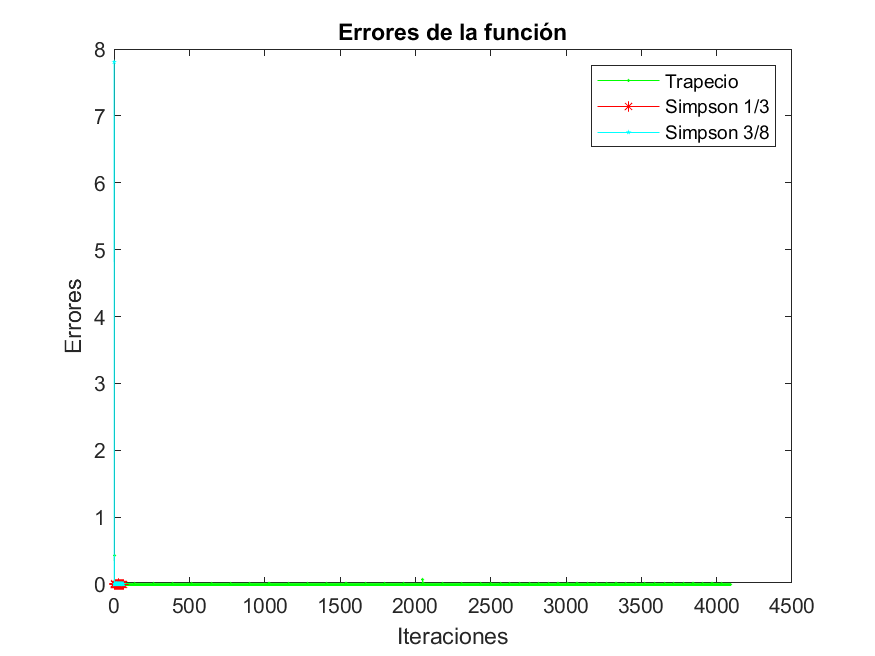
\includegraphics[scale=0.7]{Imagenes/erroresFuncion.png}
	\caption{Resultado de las aproximaciones de la prueba 1}
	\label{fig:ej}
\end{figure}


\subsubsection{Segunda Prueba}

\par Para la segunda prueba se cambio los parámetros iniciales: a=2 y b=7, junto con una tolerancia de $10^{-8}$. Con esto se obtuvo los siguientes resultados.

\begin{table}[htp]
	\centering
	\begin{tabular}{ |c|c|c|c|}
		\hline
		\textbf{Método} & \textbf{Aproximación} & \textbf{Error} & \textbf{Iteraciones} \\
		\hline
		Trapecio & 88.894188 & $8.7 \cdot 10^{-9}$ & 12.787  \\
		\hline
		Simpson 1/3 & 88.894185 & $8.6 \cdot 10^{-9}$ & 251  \\
		\hline
		Simpson 3/8 & 8.894185 & $8.6 \cdot 10^{-9}$ & 251 \\
		\hline
	\end{tabular}
	\caption{Tabla de resultados para la segunda prueba}
	\label{tab:tab3}
\end{table}


\begin{figure}[!ht]
	\centering
	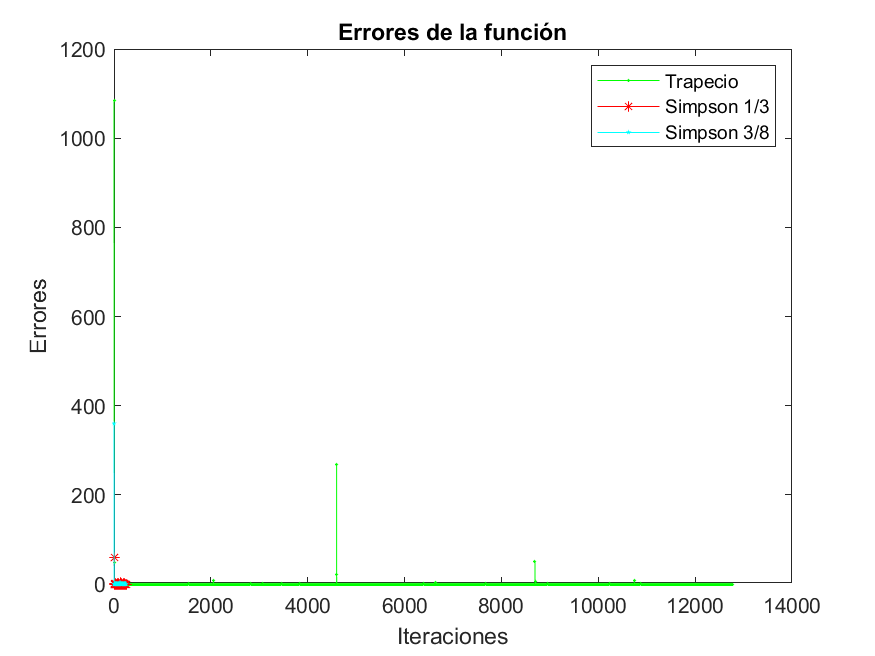
\includegraphics[scale=0.8]{Imagenes/erroresFuncion2.png}
	\caption{Resultado de las aproximaciones de la prueba 2}
	\label{fig:ej}
\end{figure}

\newpage

\subsubsection{Tercera Prueba}

\par Para la tercera prueba se cambio los parametros iniciales: a=1 y b=4, junto con una tolerancia de $10^{-3}$. Con esto se obtuvo los siguientes resultados.

\begin{table}[htp]
	\centering
	\begin{tabular}{ |c|c|c|c|}
		\hline
		\textbf{Método} & \textbf{Aproximación} & \textbf{Error} & \textbf{Iteraciones} \\
		\hline
		Trapecio & -9.799697 & $4.8 \cdot 10^{-4}$ & 105  \\
		\hline
		Simpson 1/3 & -9.802113 & $7.8 \cdot 10^{-5}$ & 11  \\
		\hline
		Simpson 3/8 & -9.802113 & $7.8 \cdot 10^{-5}$ & 11 \\
		\hline
	\end{tabular}
	\caption{Tabla de resultados para la tercera prueba}
	\label{tab:tab3}
\end{table}

\begin{figure}[!ht]
	\centering
	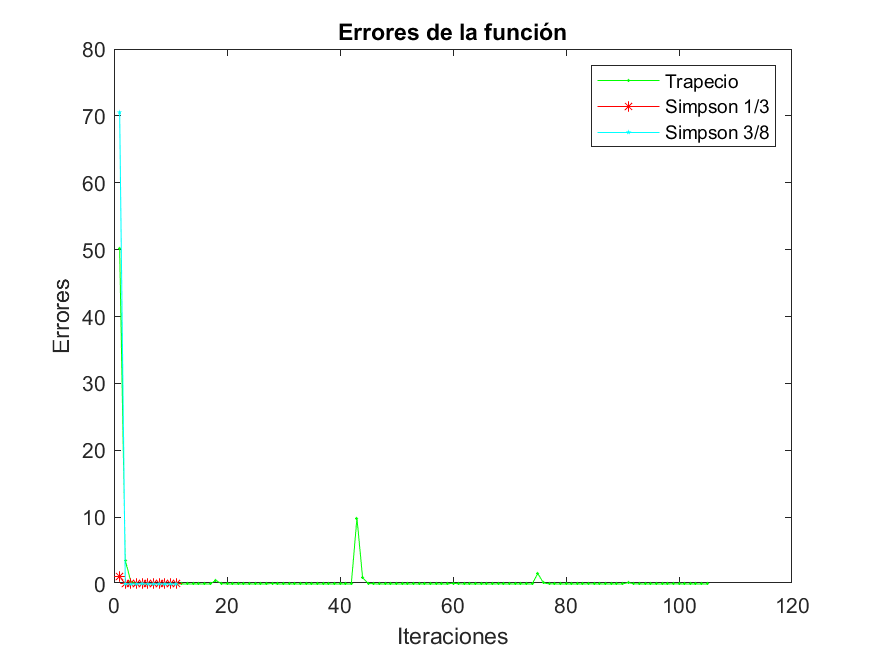
\includegraphics[scale=0.8]{Imagenes/erroresFuncion3.png}
	\caption{Resultado de las aproximaciones de la prueba 3}
	\label{fig:ej}
\end{figure}



\section{Parte II}

\subsection{Problema}

\par Se solicita  utilizar cualquier método o técnica numérica para resolver la ecuación diferencial parcial de Cromatografía de Membrana. La cromatografía es un método de separación en cual los componentes a ser separados se distribuyen en dos fases: una fija (fase estacionaria) y otra que se mueve en una determinada dirección (fase móvil). Las ventajas de utilizar una membrana para el proceso de separación es una transferencia de masa rápida, el flujo a través de la membrana no está limitado por la caída de presión.

\begin{figure}[!ht]
	\centering
	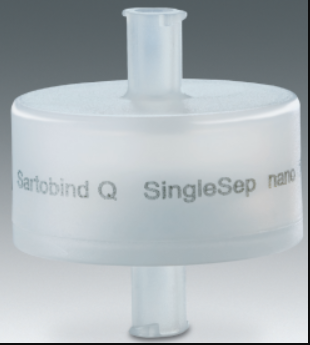
\includegraphics[scale=0.7]{Imagenes/membrana.png}
	\caption{Figura de la membrana}
	\label{fig:ej}
\end{figure}

Se modela utilizando el balance de proteínas en la fase móvil (5). La ecuación diferencial parcial para cada proteína (i=1....N) en la fase móvil. Donde $Cb_{i}$ es la concentración en el fluido y $Cb^*_{i}$ la concentración de proteína en la membrana

\begin{equation}
\begin{split}
       -D_{bi}\cdot\frac{\partial^2 Cb_{i}}{\partial z^2}+\frac{\partial Cb_{i}}{\partial z}+\frac{\partial Cb_{i}}{\partial t}+ \varepsilon(Cb_{i}-Cb^*_{i}) = 0
\end{split}
\end{equation}

\par Independiente del método utilizado para resolver la ecuación, la cromatografía de elución se lleva a cabo realizando los pasos de: inyección de la muestra, lavado de columna y
elución. Con esto se deben obtener las curvas de elución y modulación de cromatografía, junto con una gráfica en 3 dimensiones que muestre la difusión tiempo-espacio. Además, para el método utilizado debe entregar los errores (eficacia) y eficiencia (costo computacional) de este.

\subsection{Solución}

\subsubsection{Método de Diferencias Finitas}

\par  Para obtener resolver la ecuación anterior, se utiliza el método de diferencias finitas sobre ecuaciones diferenciales parciales, para esto se deben establecer las condiciones de frontera las cuales son:

\begin{itemize}
	\item Cb(z,0) = 0   $0 < z < L$;  L: Largo de la columna
	\item Cb(L,t) = 0  $0< t < tmax$; donde el tmax equivale al largo t de la matriz
	\item Cb(0,t) = funcion pulso; cuando $t < tinyeccion$; t = 2 y cuando $t > tinyeccion$, t = 0
\end{itemize}

Lo primero que se debe hacer para una ecuación utilizando diferencias finitas es discretizar la ecuación. Para la discretización del dominio se crea una matriz de $n x m$ donde n seria las veces que divide la columna (nz) y m el tiempo aproximado que nosotros le damos a que se realiza la cromatografía. Una forma de representarlo sería:

\begin{figure}[!ht]
	\centering
	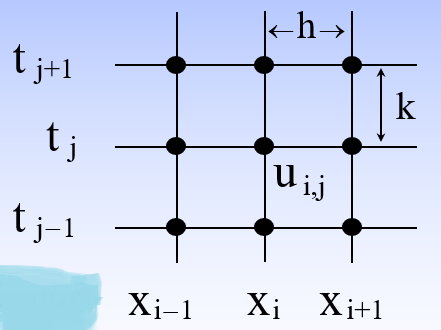
\includegraphics[scale=0.6]{Imagenes/matriz.png}
	\caption{Forma de representar la matriz}
	\label{fig:ej}
\end{figure}

\par Donde $u_{i,j}$ seria el $Cb_{i}$ de la ecuación, h y k serian dz y dt respectivamente. Y x es lo mismo que z. Para elegir los puntos en los cuales calcularemos la solución aproximada de la EDP. Al discretizar los términos tambien dividimos dz/dt obteniendo el valor B y A = (1-B), obtenemos (6):

\begin{equation}
\begin{split}
    \frac{1}{PE}\cdot\frac{Cb_{i-1,j}-2Cb_{i,j}+Cb_{i+1,j}}{h^2} + B\cdot Cb_{i-1,j-1} + A\cdot Cb_{i,j-1}
\end{split}
\end{equation}


\subsubsection{Elución y Modulación}

\par Antes de explicar la graficar se debe indicar que los parámetros nz y tiempo son muy limitados, por lo realizado en este laboratorio nz no puede ser inferior a 15 o superior a 22 y el tiempo en el cual se efectúa debe estar entre 90 y 110, para que se obtengan las curvas de elución y modulación. 

\par Para obtener la curva de elución, debe graficar según los resultados obtenidos en el último z antes de llegar al largo L de la columna (Ya que en L, el tiempo es 0) . Para la curva de modulación se debe guardar los valores de sal desde el proceso de inyección, lavado hasta el proceso de elución (se especifica mejor en el código).

\subsection{Resultados}

\par En esta sección entregaremos cada uno de los resultados obtenidos al aplicar el método de diferencias finitas en matlab.

\subsubsection{Primera prueba}

\par Como se mencionó anteriormente, el tiempo y el z debe ser los mencionados para que sea estable y se pueda obtener una gráfica entendible. Para la primera prueba se usó una matriz de ancho nz = 20 y un t = 100. Obteniendo los siguientes resultados:

\begin{figure}[!ht]
	\centering
	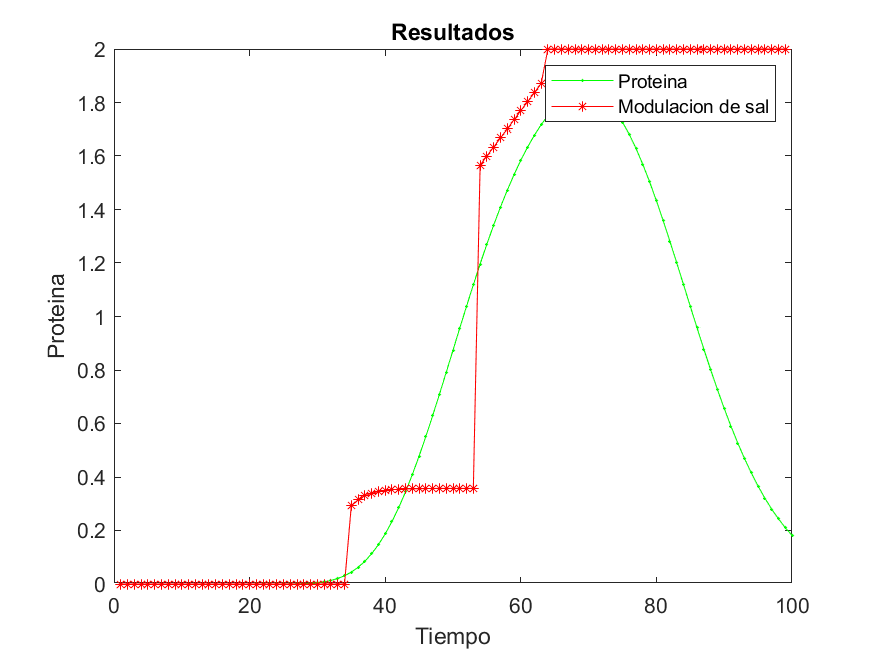
\includegraphics[scale=0.6]{Imagenes/resultado1.png}
	\caption{Resultado de las curvas de elución (verde) y modulación (rojo)}
	\label{fig:ej}
\end{figure}

\par Además de obtener la difusión tiempo y espacio para $Cb_{i}$

\begin{figure}[!ht]
	\centering
	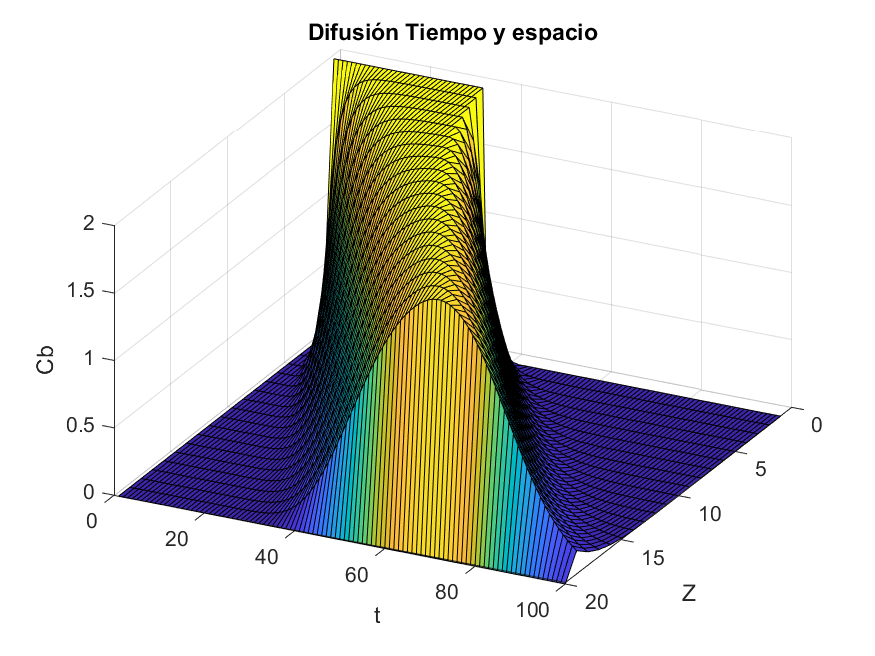
\includegraphics[scale=0.7]{Imagenes/grafico3d.png}
	\caption{Gráfico de difusión en tiempo-espacio}
	\label{fig:ej}
\end{figure}

\par Para el método utilizado de diferencias finitas se agregaron los indicadores de eficacia (error) y eficiencia (costo computacional). El error es la resta del mínimo valor con el anterior y el ultimo digito es divido por la cantidad de dígitos, el costo computacional es la cantidad de operaciones que debe realizar el computador (+,-,x,/).

\begin{table}[htp]
	\centering
	\begin{tabular}{ |c|c|c|}
		\hline
		\textbf{Método} & \textbf{Error} & \textbf{Costo Computacional}  \\
		\hline
		Direncias Finitas & 0.0354 &  23.253 \\
		\hline
	\end{tabular}
	\caption{Tabla de resultados para la primera prueba}
	\label{tab:tab3}
\end{table}

\newpage

\subsubsection{Segunda Prueba}

\par Para la segunda prueba el nz seleccionado fue 22 y para el tiempo fue 120, con lo cual se obtuvieton los siguientes resultados.

\begin{figure}[!ht]
	\centering
	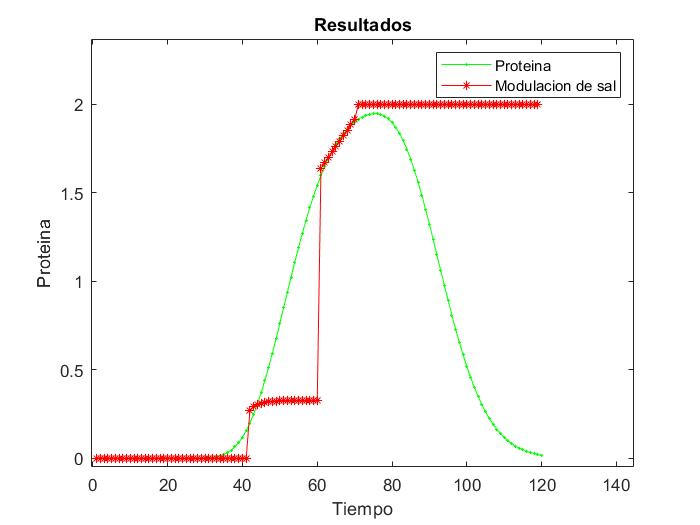
\includegraphics[scale=0.4]{Imagenes/graficoem2.jpg}
	\caption{Resultado de las curvas de elución (verde) y modulación (rojo)}
	\label{fig:ej}
\end{figure}

\newpage

\par Además de obtener la difusión tiempo y espacio para $Cb_{i}$

\begin{figure}[!ht]
	\centering
	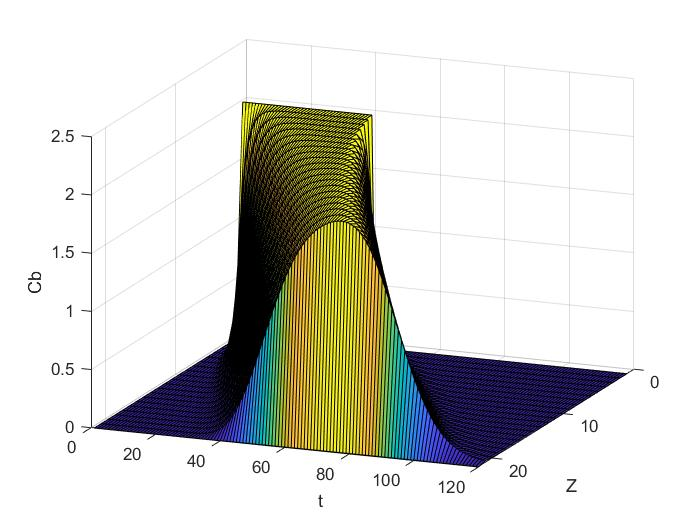
\includegraphics[scale=0.6]{Imagenes/grafico3d2.jpg}
	\caption{Gráfico de difusión en tiempo-espacio}
	\label{fig:ej}
\end{figure} 

\par Para el método utilizado de diferencias finitas se agregaron los indicadores de eficacia (error) y eficiencia (costo computacional).

\begin{table}[htp]
	\centering
	\begin{tabular}{ |c|c|c|}
		\hline
		\textbf{Método} & \textbf{Error} & \textbf{Costo Computacional}  \\
		\hline
		Direncias Finitas & 0.0265 &  31.057 \\
		\hline
	\end{tabular}
	\caption{Tabla de resultados para la primera prueba}
	\label{tab:tab3}
\end{table}




















\section{Conclusiones Globales}

\subsection{Parte I}

\par Como se pudo evidenciar en la parte I, los resultados obtenidos sobre el cálculo de la integral fueron muy precisos en los tres métodos utilizados, dándonos así el mismo valor para los 3 resultados. A pesar de que todos los métodos cumplen con el objetivo constan con una efectividad distintas debido a su manera de atacar las funciones, a excepción se puede decir del método de trapecio simples, que como se pudo apreciar en la tercera prueba, cuando se tiene una tolerancia no tan pequeña, el método no dan exactamente al resultado con un error mucho mayor. 

\subsection{Parte II}

\par  Para la parte II los resultados fueron variados. Primero se logró implementar bien el método de diferencias finitas en la ecuación diferencial parcial, ya que el gráfico de dispersión tiempo-espacio tiene gran similitud al original. Se debe destacar el número del error y el costo computacional, los cuales podían haber sido mejores.

\par La mayor dificultad fue obtener las curvas de elución y modulación. Para la curva de elución no hubo problema, ya que como se pudo apreciar en ambas pruebas se pudo lograr, pero la curva del modelamiento representa varias fallas en la parte intermedia de la curva (cuando asciende), aunque en la parte inicial y final de la curva se logra su equilibrio. Así que para esta parte del laboratorio se puede decir que se logró casi todo.

\par Mencionar que se cumplió con el objetivo principal del laboratorio que
era crear los algoritmos y analizar cada uno de sus resultados, lo cual al terminar con éxito
este laboratorio nos entregó herramientas y mayor entendimiento de cómo implementar una
abstracción matemática a un computador.


\section{Bibliografía}

\begin{itemize}
\item Sandoval,G;Cumsille,P;Rojas,O;Lienqueo,E;Conca,C.(2018), Modeling elution curves in membrane chromatography, Santiago De Chile.
\item Herrera,P.(2011), Diferencia Finitas, Santiago De Chile.
\end{itemize}

\end{document}